\documentclass[xcolor=pdflatex,dvipsnames,table]{beamer}
\usepackage{epsfig,graphicx}
\usepackage{palatino}
\usepackage{fancybox}
\usepackage{relsize}
\usepackage[procnames]{listings}

% "define" Scala
\usepackage[T1]{fontenc}  
\usepackage[scaled=0.82]{beramono}  
\usepackage{microtype} 

\sbox0{\small\ttfamily A}
\edef\mybasewidth{\the\wd0 }

\lstdefinelanguage{scala}{
  morekeywords={abstract,case,catch,class,def,%
    do,else,extends,false,final,finally,%
    for,if,implicit,import,match,mixin,%
    new,null,object,override,package,%
    private,protected,requires,return,sealed,%
    super,this,throw,trait,true,try,%
    type,val,var,while,with,yield},
  sensitive=true,
  morecomment=[l]{//},
  morecomment=[n]{/*}{*/},
  morestring=[b]",
  morestring=[b]',
  morestring=[b]"""
}

\usepackage{color}
\definecolor{dkgreen}{rgb}{0,0.6,0}
\definecolor{gray}{rgb}{0.5,0.5,0.5}
\definecolor{mauve}{rgb}{0.58,0,0.82}

% Default settings for code listings
\lstset{frame=tb,
  language=scala,
  aboveskip=3mm,
  belowskip=3mm,
  showstringspaces=false,
  columns=fixed, % basewidth=\mybasewidth,
  basicstyle={\small\ttfamily},
  numbers=none,
  numberstyle=\footnotesize\color{gray},
  % identifierstyle=\color{red},
  keywordstyle=\color{blue},
  commentstyle=\color{dkgreen},
  stringstyle=\color{mauve},
  frame=single,
  breaklines=true,
  breakatwhitespace=true,
  procnamekeys={def, val, var, class, trait, object, extends},
  procnamestyle=\ttfamily\color{red},
  tabsize=2
}

\lstnewenvironment{scala}
{\lstset{language=scala}}
{}
\lstnewenvironment{cpp}
{\lstset{language=C++}}
{}
\lstnewenvironment{bash}
{\lstset{language=bash}}
{}
\lstnewenvironment{verilog}
{\lstset{language=verilog}}
{}



\lstset{basicstyle={\footnotesize\ttfamily}}

\usetheme[height=10mm]{Rochester}

% \usetheme[height=0mm]{Rochester}
% \usecolortheme{dolphin}
% \useinnertheme{rectangles}
% \useoutertheme[footline=empty, subsection=true]{miniframes}
% \setbeamercolor{frametitle}{bg=}

\newenvironment{sample}{\VerbatimEnvironment\begin{footnotesize}\begin{semiverbatim}}{\end{semiverbatim}\end{footnotesize}}

\newenvironment{FramedSemiVerb}%
{\begin{Sbox}\begin{minipage}{0.95\textwidth}\begin{semiverbatim}}%
{\end{semiverbatim}\end{minipage}\end{Sbox}
\setlength{\fboxsep}{8pt}\fbox{\TheSbox}}

\newenvironment{FramedVerb}%
{\VerbatimEnvironment
\begin{Sbox}\begin{minipage}{0.95\textwidth}\begin{Verbatim}}%
{\end{Verbatim}\end{minipage}\end{Sbox}
\setlength{\fboxsep}{8pt}\fbox{\TheSbox}}

% \newenvironment{sample}{\VerbatimEnvironment\begin{footnotesize}\begin{Verbatim}}{\end{Verbatim}\end{footnotesize}}
\newcommand{\kode}[1]{\begin{footnotesize}{\tt #1}\end{footnotesize}}
\newcommand{\comment}[1]{{\color{Red}\it\smaller #1}}

\title{Chisel: Constructing Hardware In a Scala Embedded Language}
\author[Jonathan Bachrach et al]{Jonathan Bachrach, Huy Vo, Brian Richards, \\
Yunsup Lee, Andrew Waterman, Rimas Avizienis, \\
John Wawrzynek, Krste Asanovic}
\date{\today}
\institute[UC Berkeley]{EECS UC Berkeley}

\begin{document}

\begin{frame}
\titlepage
\end{frame}

\begin{frame}[fragile]
\frametitle{Motivation}
\begin{itemize}
\item Harder to get hardware / software efficiency gains
\item Need massive design-space exploration
\item Traditional hardware description languages are inadequate
\begin{itemize}
\item Low level
\item Poor for writing generators
\end{itemize}
\end{itemize}
\end{frame}

\begin{frame}[fragile]{The Scala Programming Language}
\begin{itemize}
\item Compiled to JVM
\begin{itemize}
\item Good performance
\item Great Java interoperability
\item Mature debugging, execution environments
\end{itemize}
\item Object Oriented
\begin{itemize}
\item Factory Objects, Classes
\item Traits, overloading etc
\end{itemize}
\item Functional
\begin{itemize}
\item Higher order functions
\item Anonymous functions
\item Currying etc
\end{itemize}
\item Extensible
\begin{itemize}
\item Domain Specific Languages (DSLs)
\end{itemize}
\end{itemize}
\end{frame}

\begin{frame}[fragile]{Chisel is ...}
\begin{itemize}
\item Best of hardware and software
\item Embedded within Scala language to leverage mindshare and language design
\item Algebraic construction and wiring
\item Hierarchical and object oriented construction
\item Abstract data types and interfaces
\item Bulk connections
\item Multiple targets
\begin{itemize}
\item Simulation and synthesis
\item Memory IP is target-specific
\end{itemize}
\end{itemize}
\end{frame}

\begin{frame}[fragile]{Primitive Datatypes}
\begin{itemize}
\item{Chisel has 4 primitive datatypes}
\begin{description}
\item[Bits]  -- raw collection of bits
\item[Fix]   -- signed fixed-point number
\item[UFix] -- unsigned fixed-point number
\item[Bool] -- Boolean value
\end{description}
\item Can do arithmetic and logic with these datatypes
\end{itemize}

\textbf{Example Literal Constructions}
\begin{scala}
val sel = Bool(false);
val a   = UFix(25);
val b   = Fix(-35);
\end{scala}
where \verb+val+ is a Scala keyword used to declare variables whose values won't change
\end{frame}

\begin{frame}[fragile]{Aggregate Data Types}

\textbf{Bundle}

\begin{itemize}
\item User-extendable collection of values with named fields
\item Similar to structs
\end{itemize}

\begin{footnotesize}
% \textbf{Bundle Example}
\begin{scala}
class MyFloat extends Bundle{
  val sign        = Bool();
  val exponent    = UFix(width=8);
  val significand = UFix(width=23);
}
\end{scala}
\end{footnotesize}

\textbf{Vec}

\begin{itemize}
\item Create indexable collection of values
\item Similar to array
\end{itemize}

\begin{footnotesize}
% \textbf{Vec Example}
\begin{scala}
val myVec = Vec(5){ Fix(width=23) }
\end{scala}
\end{footnotesize}

\end{frame}

\begin{frame}[fragile]{Example}
\begin{footnotesize}
\begin{scala}
class GCD extends Component {
  val io = new Bundle {
    val a   = UFix(16, INPUT);
    val b   = UFix(16, INPUT);
    val z   = UFix(16, OUTPUT);
    val rdy = Bool(OUTPUT); };
  val x  = Reg(resetVal = io.a);
  val y  = Reg(resetVal = io.b);
  when (x > y) {
    x := x - y;
  } .otherwise {
    y := y - x;
  }
  io.z   := x;
  io.rdy := y === UFix(0);
}
\end{scala}
\end{footnotesize}
\end{frame}

\begin{frame}[fragile]{Polymorphism and Parameterization}
\begin{itemize}
\item Chisel users can define their own parameterized functions
\begin{itemize}
\item Parameterization encourages reusability
\item Data types can be inferred and propagated
\end{itemize}
\end{itemize}

\textbf{Example Shift Register:}
\begin{scala}
def delay[T <: Bits](x: T, n: Int): T = 
  if(n == 0) x else Reg(delay(x, n – 1))
\end{scala}
where
\begin{itemize}
\item The input \verb+x+ is delayed n cycles
\item \verb+x+ can by of any type that extends from \verb+Bits+
\end{itemize}

\end{frame}

\begin{frame}[fragile]{Abstract Data Types}
\begin{itemize}
\item The user can construct new data types
\begin{itemize}
\item Allows for compact, readable code
\end{itemize}
\item Example: Complex numbers
\begin{itemize}
\item Useful for FFT, Correlator, other DSP
\item Define arithmetic on complex numbers
\end{itemize}
\end{itemize}

\begin{footnotesize}
\begin{scala}
class Complex(val real: Fix, val imag: Fix) 
    extends Bundle {
  def + (b: Complex): Complex = 
    new Complex(real + b.real, imag + b.imag);
  ...
}
val a = new Complex(Fix(32), Fix(-16));
val b = new Complex(Fix(-15), Fix(21));
val c = a + b;
\end{scala}
\end{footnotesize}

\end{frame}

\begin{frame}[fragile]{Generator}
\begin{footnotesize}
\begin{scala}
class Cache(cache_type:    Int = DIR_MAPPED,
            associativity: Int = 1,
            line_size:     Int = 128,
            cache_depth:   Int = 16,
            write_policy:  Int = WRITE_THRU
           ) extends Component {
  val io = new Bundle() {
    val cpu = new IoCacheToCPU();
    val mem = new IoCacheToMem().flip();
  }
  val addr_idx_width = log2(cache_depth).toInt
  val addr_off_width = log2(line_size/32).toInt
  val addr_tag_width = 32 - addr_idx_width - 
                         addr_off_width - 2
  val log2_assoc     = log2(associativity).toInt
  ...
  if (cache_type == DIR_MAPPED)
    ...
\end{scala}
\end{footnotesize}

\end{frame}

\begin{frame}{Related Work}

\begin{itemize}
\item SystemVerilog
\begin{itemize}
\item Lacks general purpose programming and extensibility
\end{itemize}
\item Lava
\begin{itemize}
\item Elegant but focus on spatial layout
\end{itemize}
\item Domain specific (bluespec + esterel + autoesl)
\begin{itemize}
\item Powerful but needs to match task at hand	
\end{itemize}
\item Generator language (Genesis2 + spiralFFT)
\begin{itemize}
\item Either inherit poor abstraction qualities of underlying HDL or
\item Do not provide complete solution
\end{itemize}
\end{itemize}

\end{frame}

\begin{frame}[fragile]{Fast Cycle-Accurate Simulation}

\begin{itemize}
\item Compiles to single class with \verb+clock_lo+ and \verb+clock_hi+ methods
\begin{itemize}
\item Keep state and top level io in class fields
\end{itemize}
\item Generates calls to fast multiword library using C++ templates 
\begin{itemize}
\item specializing for small word cases
\item remove branching as much as possible to utilize maximum ILP in processor
\end{itemize}
\end{itemize}

\end{frame}

\begin{frame}{Comparison with Hand-Coded Verilog}

\begin{itemize}
\item 3x reduction in lines of code for 3-stage RISC CPU
\item Chisel-generated Verilog gives comparable synthesis quality of results
\end{itemize}

\end{frame}

\begin{frame}[fragile]{Rocket Microarchitecture}

\begin{itemize}
\item 6-stage RISC integer datapath + 5-stage Vector IEEE FPU + MMU and non-blocking caches
\end{itemize}
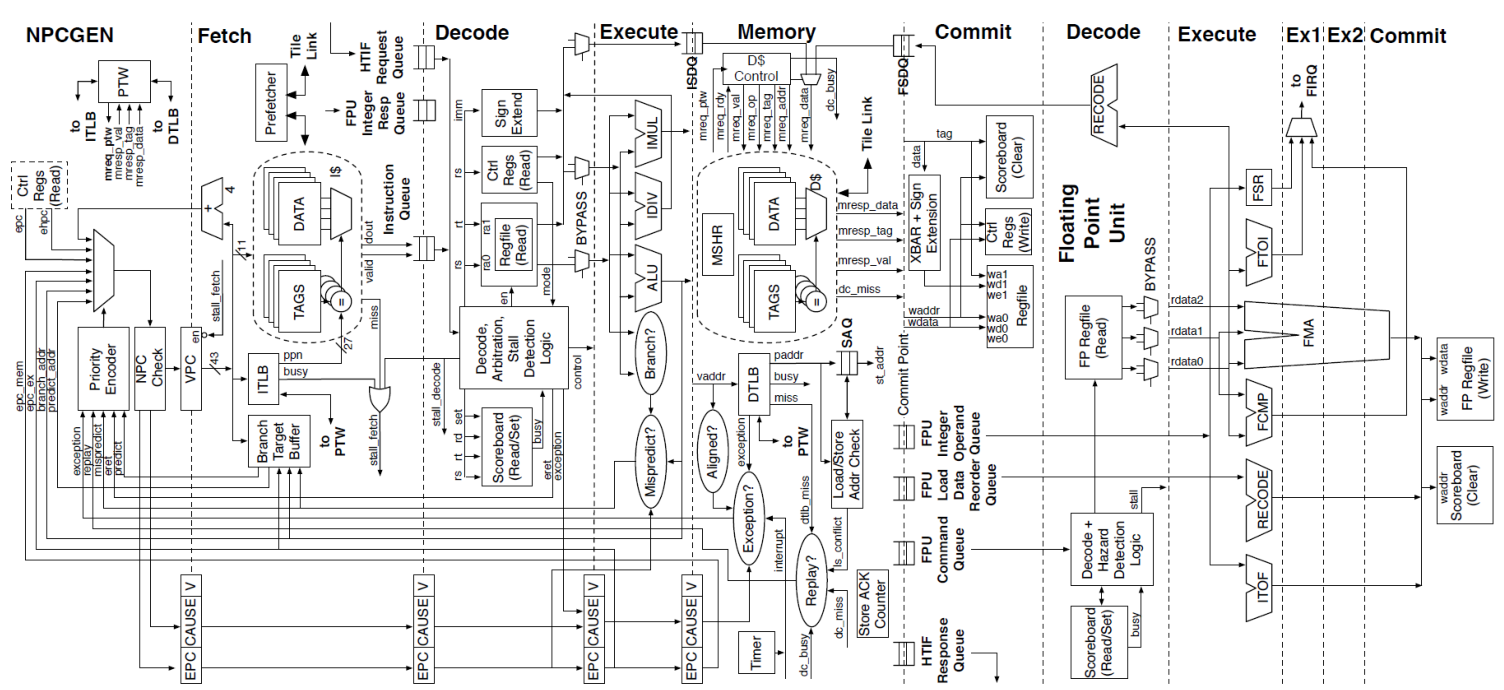
\includegraphics[width=\textwidth]{rocket-microarchitecture.pdf}

\end{frame}

\begin{frame}[fragile]{Processor Performance}

\textbf{Comparison of sim time when booting Tessellation OS}
\vskip0.5cm

\begin{tiny}
\begin{tabular}{lrrrrrr}
\textbf{Simulator} & \textbf{Compile}  & \textbf{Compile} & \textbf{Run}  & \textbf{Run} & \textbf{Total} & \textbf{Total} \\
& \textbf{Time (s)}  & \textbf{Speedup} & \textbf{Time (s)}  & \textbf{Speedup} & \textbf{Time (s)} & \textbf{Speedup} \\
\hline
VCS RTL simulator             &   22 & 1.000 & 5368 & 1.00 & 5390 & 1.00 \\ 
Chisel C++ RTL simulator & 119 & 0.184 & 575 & 9.33 & 694 & 7.77\\
Virtex-6 FPGA & 3660 & 0.006 & 76 & 70.60 & 3736 & 1.44\\
\end{tabular}
\end{tiny}

\vskip1cm

\begin{tabular}{ll}
\textbf{Name} & \textbf{Worth it if simulating more than ...} \\
\hline
Chisel C++ simulation & millions of cycles \\
FGPA emulation & billions of cycles \\
\end{tabular}

\end{frame}

\begin{frame}[fragile]{Data Parallel Processor Tape Out Results}

\begin{center}
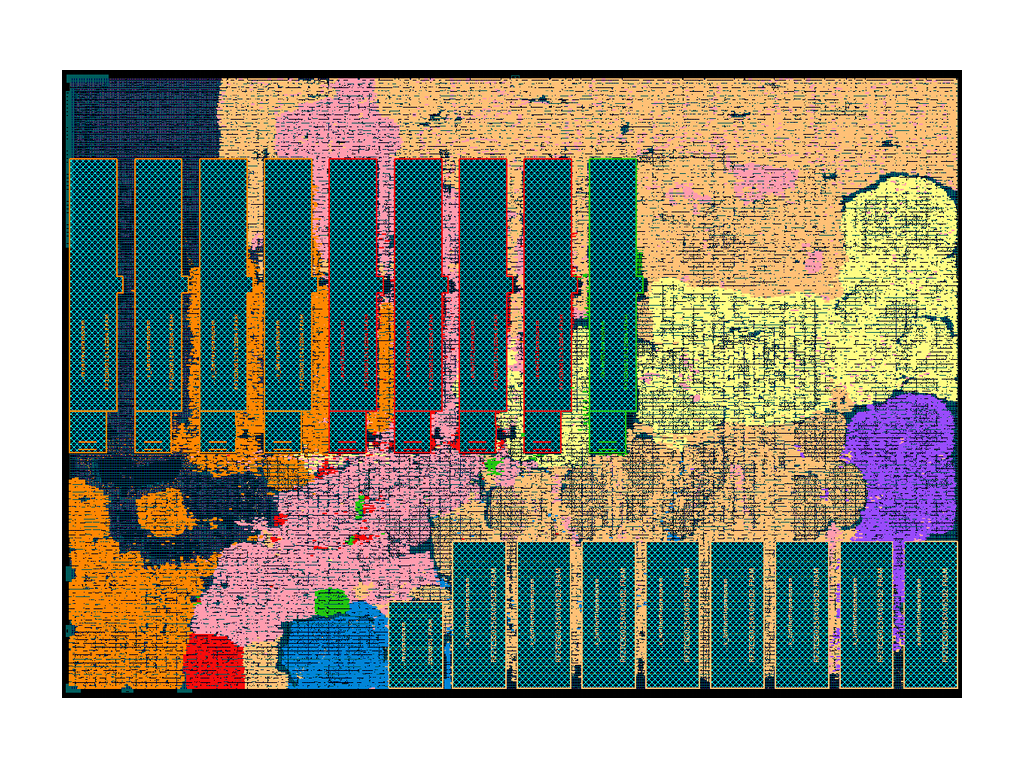
\includegraphics[height=0.75\textheight]{ibm45.png}

\begin{footnotesize}
The data-parallel processor layout results using IBM 45nm SOI 10-metal layer process using memory compiler generated 6T and 8T SRAM blocks.
\end{footnotesize}
\end{center}

\end{frame}

\begin{frame}[fragile]{Products}

\begin{itemize}
\item Open source with BSD license
\begin{itemize}
\item \verb+chisel.eecs.berkeley.edu+
\item Alpha now
\item Public Beta Available by end of summer
\end{itemize}
\item Library of components
\begin{itemize}
\item queues, decoders, encoders, popcount, scoreboards, integer ALUs, LFSR, Booth multiplier, iterative divider, ROMs, RAMs, CAMs, TLB, caches, prefetcher, fixed-priority arbiters, round-robin arbiters, IEEE-754/2008 floating-point units
\end{itemize}
\item Set of educational processors including:
\begin{itemize}
\item microcoded processor, one-stage, two-stage, and five-stage pipelines, and an out-of-order processor, all with accompanying visualizations.
\end{itemize}
\end{itemize}

\end{frame}

\begin{frame}[fragile]{Products}

\begin{itemize}
\item Automated design space exploration
\item Insertion of Activity counters for power monitors
\item Automatic fault insertion
\item Faster simulation
\item More generators
\item Little languages
\end{itemize}

\end{frame}

\begin{frame}[fragile]{Future}

\begin{itemize}
\item Demos
\begin{itemize}
\item Chisel Workflow
\item C++ Simulator with educational processors
\item Multicore RISCV on FPGA
\end{itemize}
\end{itemize}

\end{frame}

\end{document}
